\documentclass[8pt]{article}   	% use "amsart" instead of "article" for AMSLaTeX format
\usepackage{geometry}                		% See geometry.pdf to learn the layout options. There are lots.
\geometry{letterpaper}                   		% ... or a4paper or a5paper or ...
%\geometry{landscape}                		% Activate for rotated page geometry
%\usepackage[parfill]{parskip}    		% Activate to begin paragraphs with an empty line rather than an indent
\usepackage{graphicx}				% Use pdf, png, jpg, or eps§ with pdflatex; use eps in DVI mode
								% TeX will automatically convert eps --> pdf in pdflatex
\usepackage{amssymb}
\usepackage{cite}
\usepackage{subfigure}
\usepackage{float}
\usepackage{placeins}
\usepackage{hyperref}
\usepackage{placeins}
\usepackage{comment}
\usepackage{gensymb}
\usepackage{lineno}
\usepackage{authblk}
\usepackage{color}

%\date{}							% Activate to display a given date or no date

\title{Calculation of Threshold Displacement Energies in $UO_2$}
\author[1]{Benjamin Dacus}
\author[2]{Benjamin Beeler}
\author[2]{Daniel Schwen}

\affil[1]{North Carolina State University, Raleigh, NC 27695}
\affil[2]{Idaho National Laboratory, Idaho Falls, ID 83415}

\begin{document}

\begin{comment}
\author[ncst]{Benjamin Dacus}
\author[inl]{Benjamin Beeler}
\author[inl]{Daniel Schwen}
\address[inl]{Idaho National Laboratory, Idaho Falls, ID 83415}
\address[ncst]{North Carolina State University, Raleigh, NC 27695}
\end{comment}


\begin{@twocolumnfalse}
\maketitle
    \begin{abstract}
      Despite the extensive utilization of uranium dioxide ($UO_2$) as a driver fuel in commercial nuclear reactors, there is only minimal information regarding the fundamental nature of radiation damage at high temperatures, such as those experienced by the fuel under operation. In this work, molecular dynamics simulations have been performed to determine the threshold displacement energy ($E_d$) for oxygen and uranium in $UO_2$ at 1500 K. Three definitions of displacement energy were employed to fully study the nature of low energy radiation damage: 1) the probability of forming a stable Frenkel defect, 2) the probability of having the primary knock-on atom (PKA) leave its original lattice site, and 3) the number of permanently displaced atoms due to the PKA. Additionally, three unique interatomic potentials were utilized to determine uncertainties associated with potential choice in high temperature radiation damage studies in $UO_2$. This work provides critical insight into the high temperature behavior of radiation damage in $UO_2$, as well as the variation in behavior between oxygen and uranium PKAs.
    \end{abstract}
\end{@twocolumnfalse}


\clearpage
\newpage

\section{Introduction}

\hspace{5mm}
Due to its usage as a nuclear fuel, uranium dioxide ($UO_2$) has been thoroughly studied both theoretically and experimentally over the the last half-century. Utilization of this data can provide correlations for a range of thermo-mechanical behaviors, and such correlations can serve as inputs to continuum-level fuel performance modeling. Such fuel performance models \cite{williamson_et_al_2012, falcon04, bentejac2004, thouvenin2007, sercombe2009} have shown impressive accuracy in their ability to describe fuel behavior. However, fuel performance models that rely on empirical correlations are inherently limited in their applicability to the scope of the data used to construct those empirical models. In order to predict fuel behavior in scenarios outside of the existing experimental data regimes, the underlying physics of the material systems needs to be included into the fuel performance models. This can be done by informing continuum level simulations with mesoscale and atomistic data taking into account the microstructural evolution of the material.

In addition to very high neutron flux and fluence during operation, nuclear fuels are exposed to high energy fission fragments and alpha particles released during radioactive decay of fission products. The ability to quantify the damage resulting from this radiation is a critical step in describing and understanding microstructural evolution of nuclear fuel. The threshold displacement energy ($E_d$) is a critical measure of a material's response to radiation damage. The amount of damage that a material system experiences under irradiation is typically described in displacements per atom (dpa).  Models such as the Norgett-Robinson-Torrens (NRT) \cite{nrt} utilize a threshold displacement energy to calculate a given \textit{dpa} based on the material and irradiation condition.  It is thus critical to possess an accurate description of $E_d$ in order to accurately assess the number of \textit{dpa} the material system of interest experiences.

There have been several investigations over the past three decades studying $E_d$ in $UO_2$. Using transmission electron microscopy on room temperature $UO_2$ samples, Soullard \cite{soullard1977,soullard1985} determined that the threshold displacement energies in $UO_2$ are 20 eV for oxygen primary knock-on atoms (PKAs) and 40 eV for uranium PKAs. However, this work makes usage of a variety of assumptions, including the validity of the Kinchin-Pease model, extrapolation of dislocation loops to the number of point defects and that the oxygen $E_d$ is half that of the uranium $E_d$. Additionally, Soullard only reports that the uranium $E_d$ is ``on the order of 40 eV." These are the only known experimental studies on $E_d$ in $UO_2$.

Computationally, Meis and Chartier \cite{meis2005} used the sudden approximation method within the Mott-Littleton approach \cite{Litt} in order to determine $E_d$. They determined that the value of $E_d$ for oxygen PKAs ($E_d [O]$) is approximately 20 eV, and $E_d$ for uranium PKAs ($E_d [U]$) is approximately 50 eV. Molecular dynamics simulations have also been employed to investigate radiation damage in $UO_2$, although not specifically $E_d$. Van Brutzel \cite{vanbrutzel2003,vanbrutzel2006} and Martin et al \cite{martin2011} performed radiation damage simulations for PKA energies of up to 100 keV at 300 K and compared their results to the NRT correlation for an $E_d$ value of 30 eV (averaged over the experimental results of 20 eV for O and 40 eV for U). It is interesting to note that Van Brutzel determined that the linear NRT corelation was not valid at higher energies due to the recombination of defects and that the number of defects instead follows a power law, but Martin showed that a linear relationship is retained at high PKA energies. Devanathan \cite{devanathan2009} conducted 1 keV cascade simulations at 300 K utilizing five different interatomic potentials and extrapolated the displacement energy from the modified Kinchin-Pease equation \cite{kinchinpease}. Martin \cite{martin2015, martin2014} studied the effect of temperature on displacement cascades using the Morelon \cite{morelon2003} potential. The authors are unaware of any attempts to investigate the nature of $E_d$ in $UO_2$ at high temperatures. We note that all these studies employ the basic monoatomic NRT model which is not rigorously applicable to the diatomic UO$_2$,  which has two constituents that have very different $Z$ values and thus very different charged particle scattering cross sections.

Although $E_d$ has been extensively studied computationally, there still exist some discrepancies with regard to how individual researchers define $E_d$. Meis and Chartier \cite{meis2005} define $E_d$ as the "minimum energy transferred to a lattice atom along a given crystallographic direction yielding the creation of a stable Frenkel defect". However, other authors such as Devanathan \cite{devanathan1998} define the threshold displacement energy as "the minimum energy needed to displace an atom from its lattice site." This definition from Devanathan is yet unclear with respect to how displacement is defined. For instance, the energy required to remove an atom from a lattice site \textit{permanently} is higher than the energy required to remove an atom from is lattice site and have it eventually return. A more precise definition is described by Motta \cite{Motta}  where $E_d$ is "the minimum energy required to sufficiently move the atoms so that they do not return to their initial sites". It should be noted that this definition from Motta does not necessarily indicate the generation of a stable Frenkel pair. It is worth investigating all three definitions (generation of a Frenkel pair, displacement off initial lattice site, permanent displacement off initial lattice site) of the threshold displacement energy separately in order to ascertain the differences in the hopes of implementing the correct definition for the correct application.

In this study we will determine the threshold displacement energy for uranium and oxygen PKAs in $UO_2$ at 1500 K. Three different interatomic potentials will be utilized to determine uncertainties associated with potential choice in high temperature radiation damage studies in $UO_2$. The threshold displacement energy is investigated through the following definitions: 1) the probability of forming a stable Frenkel defect, 2) the probability of having the primary knock-on atom (PKA) leave its original lattice site, and 3) the number of permanently displaced atoms due to the PKA. This work provides the first high temperature investigation into the threshold displacement energy of $UO_2$.

\section{Interatomic potentials}

\hspace{5mm}
Molecular dynamics (MD) solves Newton's equations of motion on a collection of particles utilizing a potential energy function that defines the ways in which the particles interact. In this study, molecular dynamics are used to determine the threshold displacement energies. Although it is possible to determine $E_d$ from other methods like density functional theory (DFT), such \textit{ab initio}-MD methods are deemed far too computationally expensive at this stage and there exist a plethora of interatomic potentials available for the $UO_2$ system that are in common usage, particularly with regard to radiation damage simulations.

This work makes use of three distinct $UO_2$ interatomic potentials to govern particle interactions. The Basak \cite{basak}, Yamada\cite{yamada} and Yakub \cite{yakub} potentials have all been demonstrated to reproduce certain experimental properties when tested at temperatures and pressures of interest \cite{govers1,govers2,potashnikov}. The Yamada and Yakub potentials were selected specifically because of their close approximations of physical properties of $UO_2$ at 1500 K, such as the lattice parameter $a_0$, specific heat $C_p$, and the Bulk modulus $K$ \cite{govers2}. The Basak potential was selected because it is an improved fitting of the Yamada potential, created by using isothermal compressibility data in order to better model the lattice parameter and lattice expansion \cite{basak}.

These potentials in their native form do not contain a repulsive potential sufficient to model small distance interactions between atoms. For this reason, the Ziegler-Biersack-Littmark (ZBL) \cite{ZBL} potential was splined to the three separate potentials so that high energy atoms would interact with other atoms in a more physical manner. This ZBL spline occurred between 0.35 and 1.34 {\AA} for the O-O interaction, 1.7 and 2.12  {\AA} for the U-U interaction, and 0.64 and 1.09  {\AA} for the U-O interaction. At these interatomic separation distances the respective potential energy contributions well exceed the thermal energies at the temperatures of interest. We therefore expect the properties of the potentials for non-irradiation observables to be unaffected by this modification.

\section{Computational details}

\hspace{5mm}

Molecular dynamics simulations are performed with the LAMMPS \cite{lammps} software package. Threshold displacement energies are typically obtained through supplying a primary knock-on atom (PKA) with an additional amount of kinetic energy and the subsequent interaction of the PKA with other atoms in a lattice. By systematically increasing the PKA energy over a prescribed range of energies, the relationship of the number of defects produced to PKA energy can be developed. In a system at 0 K utilizing low energy PKAs, this relationship would be a step function, where below a critical PKA energy zero defects are generated and above that critical energy a single defect is generated. However, in a system at high temperature the thermal fluctuations smooth out this step function and create a continuous probability curve. Thus, a range of PKA energies are required to adequately sample the probability distribution for defects as a function of PKA energy.

Simulations were performed at low PKA energies in the 5-65 eV range in increments of 5 eV and a subset of simulations were performed at higher PKA energies in the 150-200 eV range in order to fully investigate the breadth of atomic displacements in the system. The simulations at low energies consisted of 6144 particles while the higher energy PKAs utilized a supercell with 32,928 atoms such that there was an equivalent energy per atom ratio to the lower energy runs. Systems were initialized and minimized at 0 K. The temperature was then increased to 1500 K and the system was equilibrated in an NPT ensemble. This temperature was chosen as it is a realistic fuel temperature. A PKA is introduced into the equilibrated system, the timestep is reduced to $5\cdot10^{-5}$ ps and the system is allowed to evolve in an NVE ensemble for 20000 timesteps (1 ps), after which the timestep is increased to $5\cdot10^{-4}$ ps and the simulation is allowed to evolve for another 9000 timesteps (4.5 ps), for a total post-PKA relaxation time of 5.5 ps.  Subsequently, the systems are quenched to 0 K over approximately 14 ps and their configurations energetically minimized using a conjugate gradient minimizer for ease of post-processing.

PKAs were initialized in the following directions: [110], [130], [141], [214], [232], and [313]. These directions were selected because they offer a range of both low and high symmetry directions. Additionally, both U and O atoms were utilized as the PKA in each of these directions. For each unique simulation setup for a given direction, PKA species, PKA energy and potential, 40 independent simulations were performed via random number initialization of velocities to ensure the statistical significance of the data set. Thus, a total of 19,440 simulations were performed in the course of this work.

Atomic positions were output at various times throughout the simulation in order to accurately investigate all three definitions of the threshold displacement energy. For the first definition (generation of a Frenkel pair), the Voronoi package within the LAMMPS code \cite{lammps,voro} was utilized. This package creates a Voronoi tesselation at an initial stage and determines if additional atoms are present in the cell (or atoms have left the cell) at the end of the simulation, allowing for a direct way to determine vacancies and interstitials. For the second and third definitions (displacement of PKA off initial lattice site and permanent displacement off initial lattice site), atomic positions were output once the system reached a thermal state, indicating the end of the thermal spike. It should be noted why atomic positions were output immediately after the return to a thermal state and not at the end of the simulation. Oxygen interstitials diffuse rapidly within these systems, and when one is trying to determine the number of atoms that have been displaced in a system, rapid O interstitial diffusion will artificially inflate this number, due to dumbbell diffusion moving atoms in a chain-like fashion and self-healing of O interstitials \cite{ajay}. Thus, in order to obtain the number of displaced atoms due solely to the damage cascade, systems are quenched immediately following the dissipation of the thermal spike. The specification for the determination of a thermal state is when the sum of excess kinetic energy, $\sum (KE-1 eV)$, of all atoms above 1 eV is less than 5 eV. In systems with higher energy PKAs, there are approximately 5x more atoms, thus the criterion was increased from 5 eV to 25 eV. These specifications are sufficiently strict to ensure that the PKA energy spike has dissipated. Figure \ref{fig:KE} shows the total excess kinetic energy of atoms above 1 eV as a function of time following the introduction of the PKA. The thermal state is reached around time step 3,500 (0.175 ps) where the sum of excess kinetic energy of all particles above 1 eV was equal to 5 eV. The figure is made from an arbitrary run in which the PKA was a 50 eV uranium atom, hence the initial energy of approximately 50 eV.

\begin{figure}[H]
\centering
	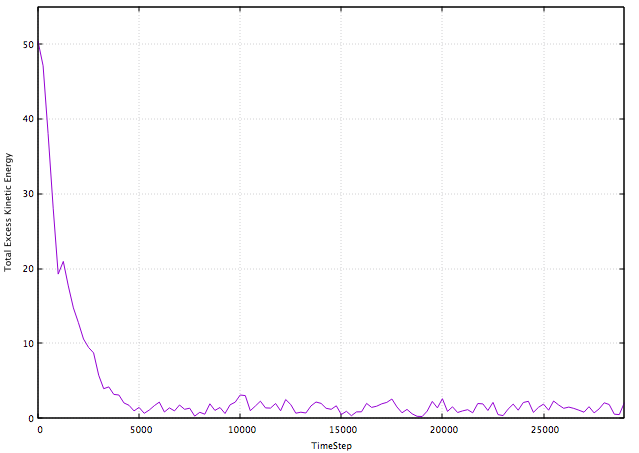
\includegraphics[width=0.6\linewidth]{ETN.png}
	\caption{Total Excess kinetic energy for all atoms above 1 eV versus time following the introduction of the PKA.}
	\label{fig:KE}
\end{figure}

\section{Results}

\subsection{Probability of Frenkel pair formation}

\hspace{5mm}

The probability of Frenkel pair formation as a function of energy for U PKAs is shown in Fig. \ref{fig:fpu}. Probabilities are observed to be zero up to approximately 25 eV for all interatomic potentials and directions. Above 20 eV, probabilities become non-zero and there is a clear directional dependence in the probability curves. The [214] direction consistently exhibits the lowest probability for Frenkel pair formation for all three potentials, while the [130] and [141] directions consistently have the highest probability of Frenkel pair formation. Thus, it is easiest to generate defects from PKAs in the [130] and [141] directions and most difficult to generate defects for PKAs in the [214] direction. Generally, excellent agreement is observed between the potentials. Utilizing the definition of $E_d$ as the lowest energy at which defect formation occurs, the displacement energy for uranium PKAs ($E_d [U]$) is 30 eV for the Basak and Yakub potentials, and 25 eV for the Yamada potential. This is substantially lower than the experimentally reported value of 40 eV \cite{soullard1977,soullard1985}.

It can often be valuable to generate an average probability curve and analyze the median of this curve (the point where the probability becomes greater than 0.5). This value for $E_{d}$ is not a quantity directly comparable to experiment, but is likely the more appropriate value for usage in the NRT equation \cite{nordlund2006, beelertde}. Thus, the results for the six PKA directions are linearly averaged to create a single probability curve for Frenkel pair formation as a function of PKA energy. The median value for $E_d [U]$ is 54 eV for Basak, 54 eV for Yakub, and 55.5 eV for Yamada. Interestingly, this interpretation for $E_{d}$ compares very favorably to the computational studies of Meis \cite{meis2005}. It should be noted that given this limited set of PKA directions, a true crystallographically averaged Frenkel pair formation probability curve would likely be different in nature. However, this simplified exercise can still provide a valuable approximation for the average behavior of U PKAs in the $UO_{2}$ system.

\begin{figure*}[h]
 \centering
 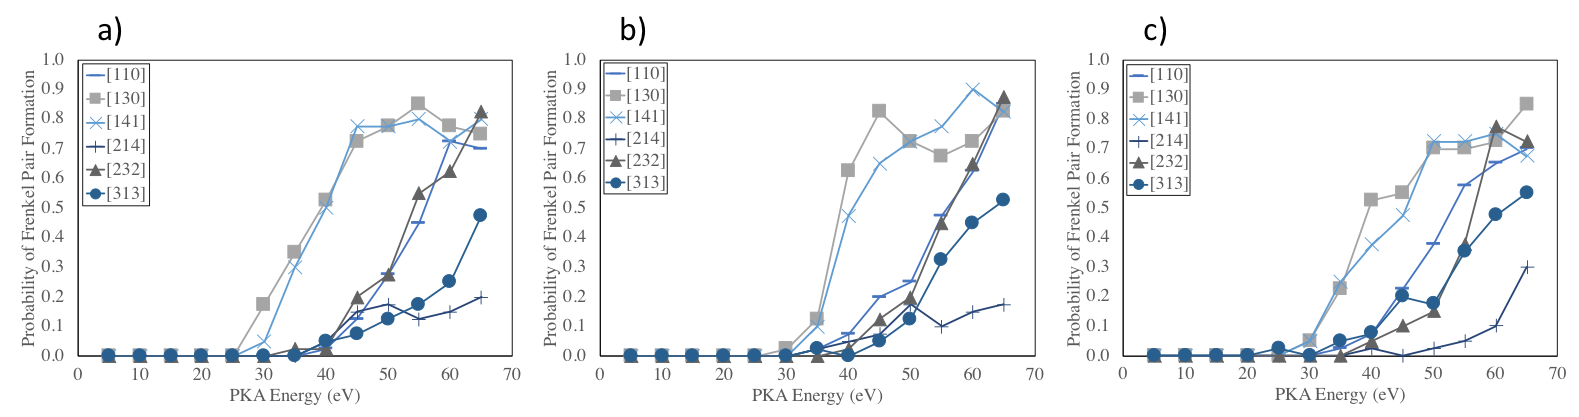
\includegraphics[width=1.0\textwidth]{FP_U.png}
 \caption{Probability of Frenkel pair formation as a function of PKA energy in $UO_2$ due to uranium PKAs in the [110], [130], [141], [214], [232] and [313] directions for the a) Basak, b) Yakub and c) Yamada potentials.  }
 \label{fig:fpu}
\end{figure*}

The probability of Frenkel pair formation as a function of energy for O PKAs is shown in Fig. \ref{fig:fpo}. Probabilities are consistently below 0.1 for all PKA energies investigated in this range. Oxygen PKAs at these low energies are unable to transfer sufficient energy to displace uranium atoms, thus only O defects can be formed. Albeit very minimal, probabilities do become non-zero near a PKA energy of 20 eV. Utilizing the definition of $E_d$ as the lowest energy at which defect formation occurs, the displacement energy for oxygen PKAs ($E_d [O]$) is is 20 eV for the Basak potential and 30 eV for both the Yakub and Yamada potentials. This can be viewed as in concordance with the experimentally observed $E_d [O]$ of 20 eV \cite{soullard1977,soullard1985}. No observable directional dependence can be elucidated from these results, as the statistical noise from this sample is equal to the magnitude of the probabilities. Similarly, comparisons of potentials in untenable due to the rare Frenkel pair formation events.

Given that the probability of Frenkel pair formation does not exceed 0.1 for the range of PKA energies, the construction of a directionally-averaged probability curve (in order to obtain the PKA energy where the probability becomes greater than 0.5) is meaningless.

\begin{figure*}[h]
 \centering
 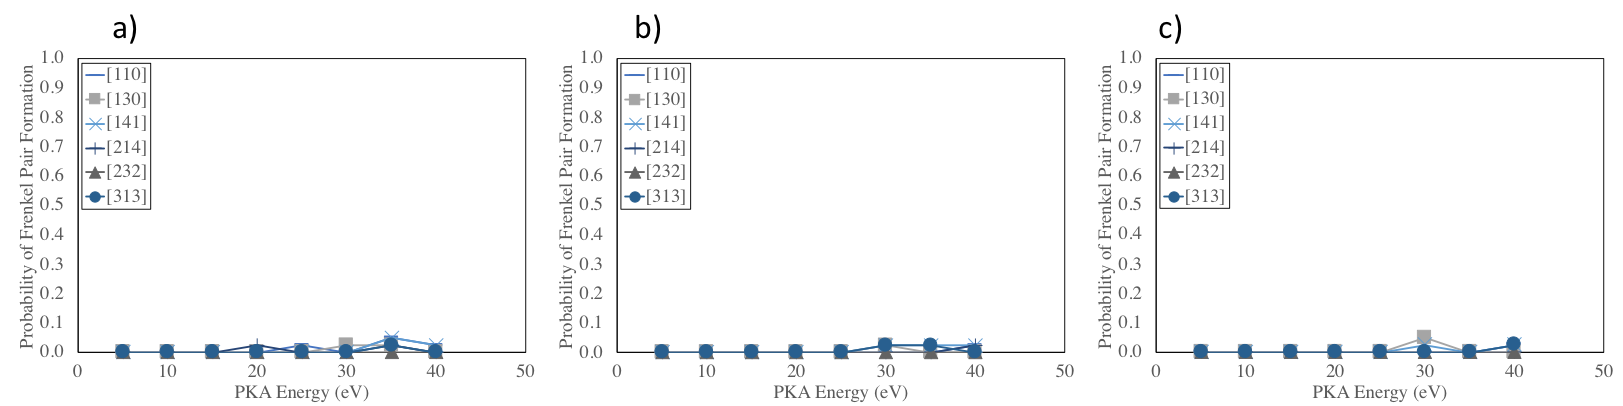
\includegraphics[width=1.0\textwidth]{FP_O.png}
 \caption{Probability of Frenkel pair formation as a function of PKA energy in $UO_2$ due to oxygen PKAs in the [110], [130], [141], [214], [232] and [313] directions for the a) Basak, b) Yakub and c) Yamada potentials.  }
 \label{fig:fpo}
\end{figure*}

\FloatBarrier

\subsection{Probability of lattice site displacement}
\hspace{5mm}
The probability of the PKA leaving its lattice site in $UO_2$ for uranium PKAs is shown in Fig. \ref{fig:latu}. It is observed that U PKAs can be displaced from their lattice site at an energy as low as 15 eV. It should be emphasized that this does not denote the generation of a defect or a permanent displacement of an atom off of its lattice site, simply that the PKA achieved a maximum displacement sufficient to be classified as no longer on its original lattice site. It makes qualitative sense, provided the nature of the definition, that the observed energies for non-zero probabilities in Fig. \ref{fig:latu} are much lower than in Fig. \ref{fig:fpu}. The highest probabilities of PKA displacement are observed for the [130] and [141] directions, similar to the results in Fig. \ref{fig:latu}. These directions show a 100{\%} likelihood of PKA displacement above an energy of 20 eV. Interestingly, the [110] direction exhibits the lowest probability of PKA displacement. Thus one can conclude from Fig. \ref{fig:fpu} and Fig. \ref{fig:latu} that although it is more difficult to displace an U atom from its lattice site in the [110] direction, there is a significant probability of that atom forming a stable Frenkel pair. This is not the case for the [214] direction, where is it moderately easy to displace an atom from its lattice site, but that atom is very unlikely to form a stable Frenkel pair. Excellent agreement is shown across all three potentials for the magnitude and the relative probabilities of PKA directions. Linearly averaging over the set of PKA directions in Fig. \ref{fig:latu} allows for the creation of a single probability curve for PKA lattice site displacement as a function of PKA energy. The single probability curve enables us to obtain the PKA energy where it is probable to displace a U atom from its lattice site. This formalism of $E_d [U]$ is 23.1 eV, 25.5 eV and 24.6 eV for the Basak, Yakub and Yamada potentials, respectively.

\begin{figure*}[h]
 \centering
 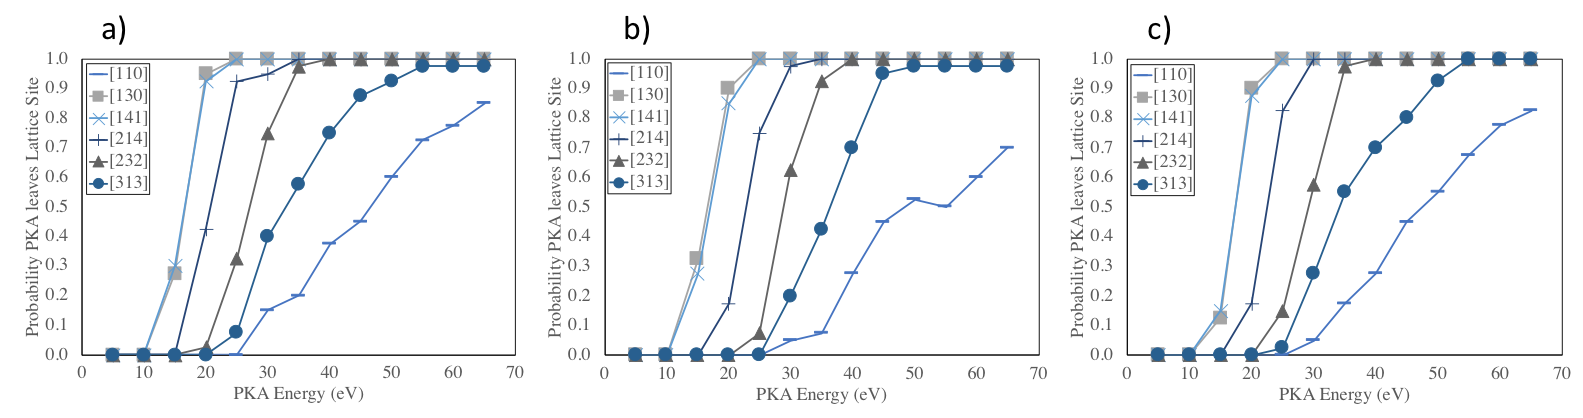
\includegraphics[width=1.0\textwidth]{lat_U.png}
 \caption{Probability of PKA leaving lattice site in $UO_2$ for uranium PKAs in the [110], [130], [141], [214], [232] and [313] directions for the a) Basak, b) Yakub and c) Yamada potentials.  }
 \label{fig:latu}
\end{figure*}

The probability of the PKA leaving its lattice site in $UO_2$ for oxygen PKAs is shown in Fig. \ref{fig:lato}. It is observed that O PKAs can be displaced from their lattice site at an energy as low as 10 eV. The highest probability of PKA displacement is observed for the [110] direction while the lowest probability of PKA displacement is observed for the [232] direction. This directional dependence is consistent over the three interatomic potentials. However, there is a noticeable difference in the magnitude of the displacement probabilities for the Yamada potential when compared to the Basak and Yakub potentials. The PKA displacement probability curves are shifted to the right for the Yamada potential, suggesting a greater difficulty of moving the O PKA from its lattice site. The data in Fig. \ref{fig:lato} is utilized to construct a single probability curve for PKA lattice site displacement as a function of PKA energy. Taking the median of this data, the $E_d [O]$ is 14.6 eV, 16.4 eV and 19.5 eV for the Basak, Yakub and Yamada potentials, respectively. This more clearly illustrates the shift right of the data of the Yamada potential.

\begin{figure*}[h]
 \centering
 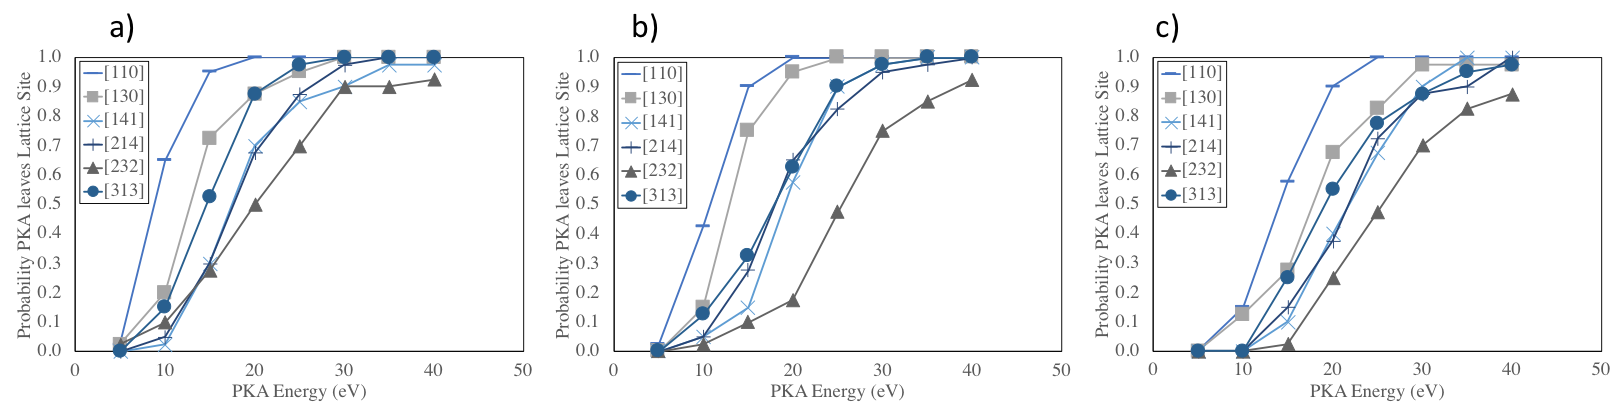
\includegraphics[width=1.0\textwidth]{lat_O.png}
 \caption{Probability of PKA leaving lattice site in $UO_2$ for oxygen PKAs in the [110], [130], [141], [214], [232] and [313] directions for the a) Basak, b) Yakub and c) Yamada potentials.  }
 \label{fig:lato}
\end{figure*}

\FloatBarrier

\subsection{Permanent displacement of atoms}
\subsubsection{Displaced oxygen atoms}
\hspace{5mm}

The average number of oxygen atoms permanently displaced per U PKA as a function of PKA energy is shown in Fig. \ref{fig:dispou}. Permanent displacement of O atoms begins at a PKA energy of approximately 20 eV. Although there exist directional dependencies for each individual potential, a general trend for high or low displacement directions across all potentials is not observable. A clear observation is the distinct differences between the three potentials. The Basak and Yamada potentials display similar behavior, while the Yamada potential predicts significantly more displaced O atoms for a U PKA of a given energy. To more clearly illustrate this phenomenon, the results for each potential are averaged over the investigated directions. At a U PKA energy of 60 eV, the directionally-averaged number of displaced O atoms per U PKA is 4.5, 3.4 and 8.1 for the Basak, Yakub and Yamada potentials, respectively. It should be emphasized that this does not necessarily indicate the generation of a Frenkel pair, but only the permanent displacement of an atom off of its original lattice site.

\begin{figure*}[h]
 \centering
 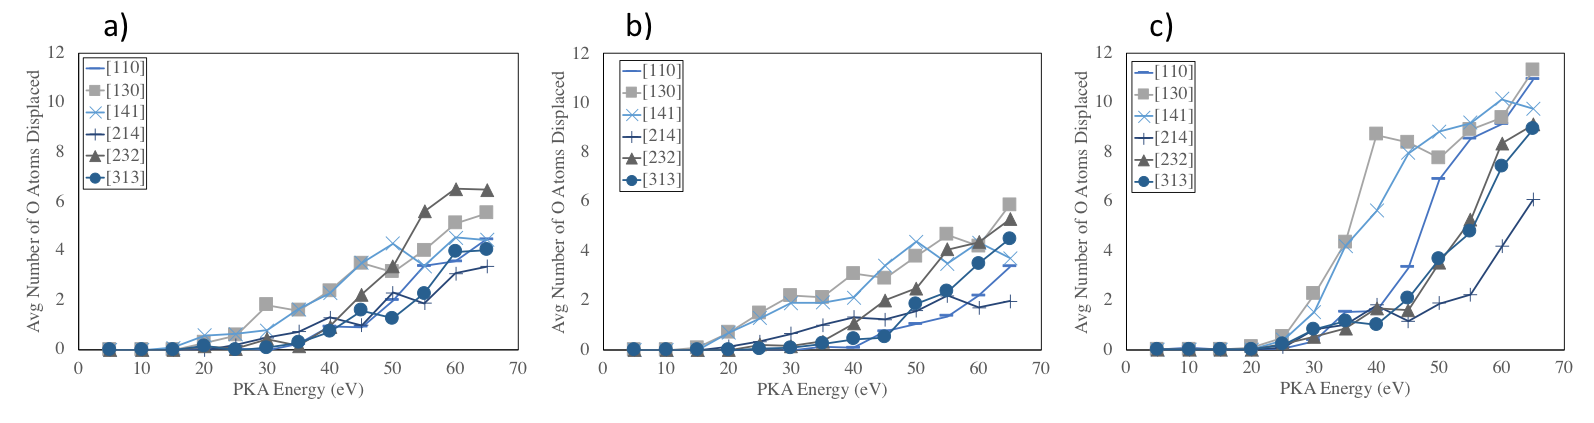
\includegraphics[width=1.0\textwidth]{dispO_U.png}
 \caption{Average number of oxygen atoms displaced by a U PKA as a function of PKA energy in $UO_2$ in the [110], [130], [141], [214], [232] and [313] directions for the a) Basak, b) Yakub and c) Yamada potentials.  }
 \label{fig:dispou}
\end{figure*}

The average number of oxygen atoms permanently displaced per O PKA as a function of PKA energy is shown in Fig. \ref{fig:dispoo}. Permanent displacement of atoms begins at an O PKA energy of approximately 20 eV. It is interesting to note that the minimum required energy to permanently displace an O atom from its lattice site is independent of whether the PKA is a U or an O atom. The [232] direction consistently exhibits the fewest number of oxygen atoms displaced per PKA across all potentials. The [110] O PKA direction leads to the highest number of displaced O atoms for the Basak and Yakub potentials, while no single high displacement direction exists for the Yamada potential. Additionally, the magnitude of the displaced O atoms is less for the Yamada potential than for the Basak and Yakub potentials. The results for each potential are averaged over the investigated directions. At an O PKA energy of 40 eV, the directionally-averaged number of displaced O atoms per O PKA is 1.6, 1.5 and 1.1 for the Basak, Yakub and Yamada potentials, respectively.

\begin{figure*}[h]
 \centering
 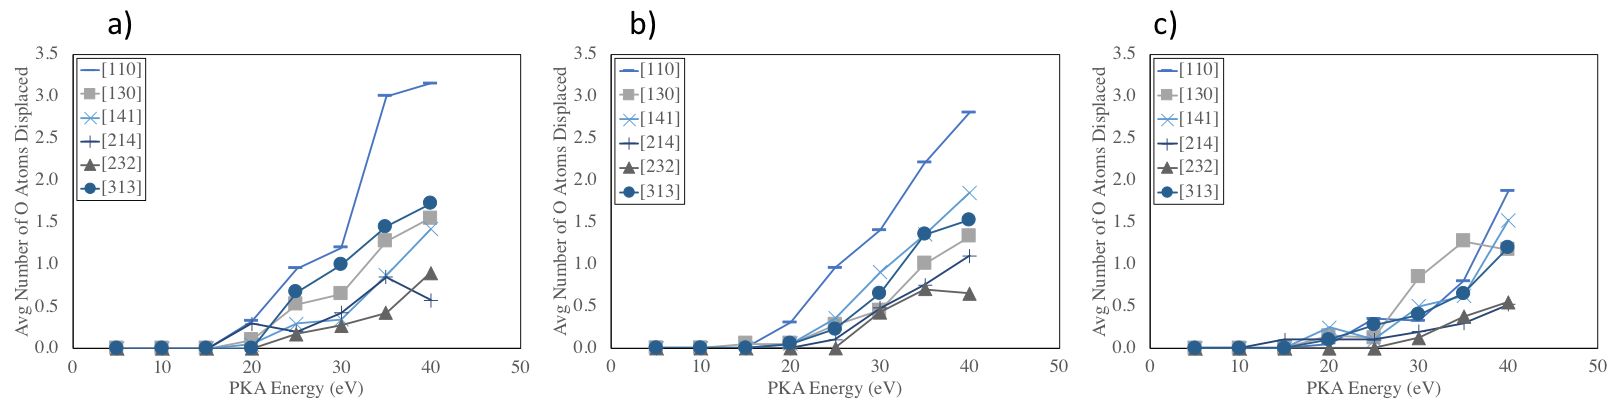
\includegraphics[width=1.0\textwidth]{dispO_O.png}
 \caption{Average number of oxygen atoms displaced by an O PKA as a function of PKA energy in $UO_2$ in the [110], [130], [141], [214], [232] and [313] directions for the a) Basak, b) Yakub and c) Yamada potentials.   }
 \label{fig:dispoo}
\end{figure*}

\FloatBarrier

\subsubsection{Displaced uranium atoms}
\hspace{5mm}

The average number of uranium atoms permanently displaced per U PKA as a function of PKA energy is shown in Fig. \ref{fig:dispuu}. Permanent displacement of atoms begins at a PKA energy of approximately 30 eV. Comparing to Fig. \ref{fig:dispou}, it requires an additional 10 eV of kinetic energy for a U atom to permanently displace another U atom, than for that U atom to displace an O atom. The [130] and [141] directions show the highest number of displaced U atoms, which is in agreement with the results in Fig. \ref{fig:fpu} on Frenkel pair generation. The fewest U atoms are displaced for PKAs in the [214] direction, which is also in agreement with Fig. \ref{fig:fpu}. There is a general agreement on directional dependence and on the magnitude of displacements for all three potentials. For a U PKA of 60 eV, the directionally-averaged number of displaced U atoms per U PKA is 1.3, 1.1 and 1.2 for the Basak, Yakub and Yamada potentials, respectively. Comparing to Fig. \ref{fig:dispou}, a U PKA of 60 eV will permanently displace approximately 4 times, 3 times or 8 times as many O atoms as U atoms for the Basak, Yakub and Yamada potentials, respectively.

Permanently displaced U atoms due to an O PKA are not shown in this section, as the low energy O PKAs did not possess sufficient kinetic energy to displace a U atom from its original lattice site.

\begin{figure*}[h]
 \centering
 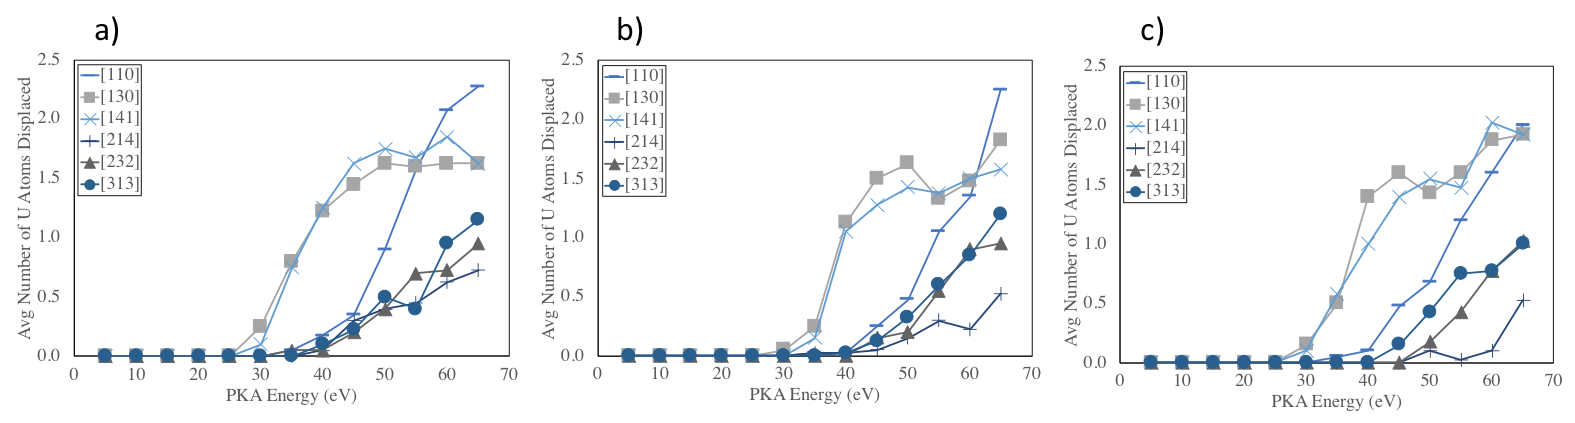
\includegraphics[width=1.0\textwidth]{dispU_U.png}
 \caption{Average number of uranium atoms displaced by a U PKA as a function of PKA energy in $UO_2$ in the [110], [130], [141], [214], [232] and [313] directions for the a) Basak, b) Yakub and c) Yamada potentials.   }
 \label{fig:dispuu}
\end{figure*}

\FloatBarrier

\subsection{High energy oxygen PKA}
\hspace{5mm}

In order to investigate the displacement of uranium atoms from an oxygen PKA, high energy (150-200 eV) oxygen PKAs were utilized. As such, a full analysis of each formalism of the displacement energy was performed for the high energy O PKAs. Figure \ref{fig:fpoe} shows the probability of Frenkel pair formation as a function of O PKA energy. For each potential, there is a slight positive trend of increasing defect probability with increasing PKA energy. Significantly, the Yamada potential predicts a dramatically higher Frenkel pair formation probability than either the Basak or Yakub potentials. At 200 eV, average probability of defect formation is 0.28, 0.26, and 0.72 for the Basak, Yakub and Yamada potentials, respectively. Thus, the Yamada potential predicts that a O PKA will produce approximately 2.5 times more Frenkel pairs than the same O PKA as predicted via the Basak or Yakub potentials. This substantial difference underlines the importance of understanding a given potential's behavior when conducting radiation damage simulations, given that similar potentials can produce dramatically different results. When comparing higher energy O PKAs in Fig. \ref{fig:fpoe} to lower energy U PKAs in Fig. \ref{fig:fpu}, it is observed that low energy U PKAs are still more likely to produce Frenkel pairs over these energy ranges (with the exception of results concerning the Yamada potential).

\begin{figure*}[h]
 \centering
 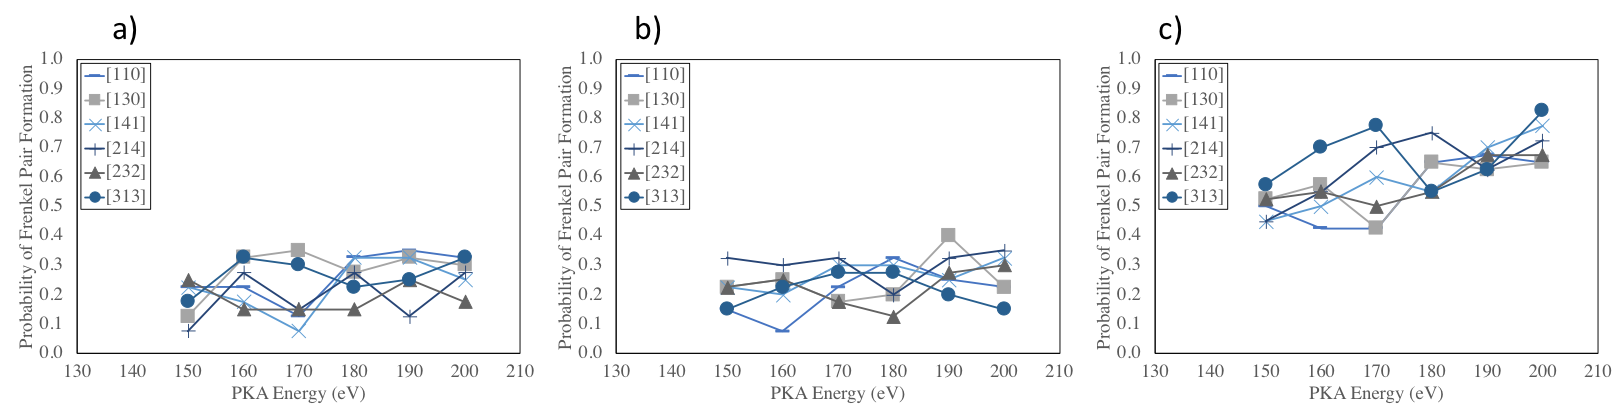
\includegraphics[width=1.0\textwidth]{FP_OE.png}
 \caption{Probability of Frenkel pair formation as a function of PKA energy in $UO_2$ due to O PKAs in the [110], [130], [141], [214], [232] and [313] directions for the a) Basak, b) Yakub and c) Yamada potentials.  }
 \label{fig:fpoe}
\end{figure*}

Table \ref{tab:dispU} shows the average number of displaced uranium atoms due to the high energy oxygen PKA. No uranium atoms were displaced in the  [110], [130], and [141] PKA directions, thus they are excluded from the table. The O PKA energy range tested encompasses the minimum energy needed to transfer approximately 50 eV to the uranium atoms (with a direct collision). Due to this fact, the average number of uranium atoms displaced is very small, as at most a single uranium atom can be displaced in a given simulation. Additionally, there is not a monotonic increase of displacement probability. As U displacements from this energy range of O PKAs are rare events and thermal fluctuations are high in these systems (simulation temperature of 1500 K), it is reasonable that there is significant statistical noise in the results. Although not statistically significant, the most likely PKA direction for U displacements is the [232] direction, and it is found that the Yakub potential is the most likely to show U displacements from these high energy O PKAs.


\begin{table}[H]
	\center
	\begin{tabular}{|c||c|c|c|}
		\hline
		 O PKA Energy (eV) & [214] & [232] & [313]\\
		\hline\hline
		 & 0 & 0 & 0\\
		150 & \textbf{0} & \textbf{0.075} & \textbf{0}\\
		 & \textit{0} & \textit{0} & \textit{0}\\
		\hline
		 & 0 & 0 & 0\\
		160 & \textbf{0} & \textbf{0} & \textbf{0}\\
		 & \textit{0} & \textit{0} & \textit{0}\\
		\hline
		 & 0 & 0.05 & 0\\
       		170 & \textbf{0} & \textbf{0.025} & \textbf{0.1}\\
		 & \textit{0} & \textit{0} & \textit{0}\\
		\hline
		 & 0 & 0.05 & 0\\
      		180 & \textbf{0} & \textbf{0} & \textbf{0.05}\\
		 & \textit{0} & \textit{0} & \textit{0}\\
		\hline
		 & 0.05 & 0.175 & 0\\
       		190 & \textbf{0} & \textbf{0.025} & \textbf{0.1}\\
		 & \textit{0} & \textit{0} & \textit{0}\\
		\hline
		 & 0 & 0.15 & 0\\
       		200 & \textbf{0.05} & \textbf{0.025} & \textbf{0}\\
		 & \textit{0} & \textit{0.05} & \textit{0}\\
		 \hline
	\end{tabular}
	\caption{Average Number of Displaced Uranium Atoms by High Energy Oxygen PKA as a function of PKA energy and direction. The potentials are denoted by font styles: Basak, \textbf{Yakub}, and \textit{Yamada}.}
	\label{tab:dispU}
\end{table}

Fig.\ref{fig:dispoe} shows the average number of displaced oxygen atoms due to the high energy oxygen PKAs. Similar to Fig. \ref{fig:fpoe} and Fig. \ref{fig:dispoo}, there is a positive trend of increasing number of displaced O atoms with increasing O PKA energy. Furthermore, the Yamada potential shows the highest number of displaced O atoms, while the Basak and Yakub show generally similar quantities of displaced O atoms. For a 200 eV O PKA, the average number of displaced O atoms is 19, 15 and 25 for the Basak, Yakub and Yamada potentials, respectively.

\begin{figure*}[h]
 \centering
 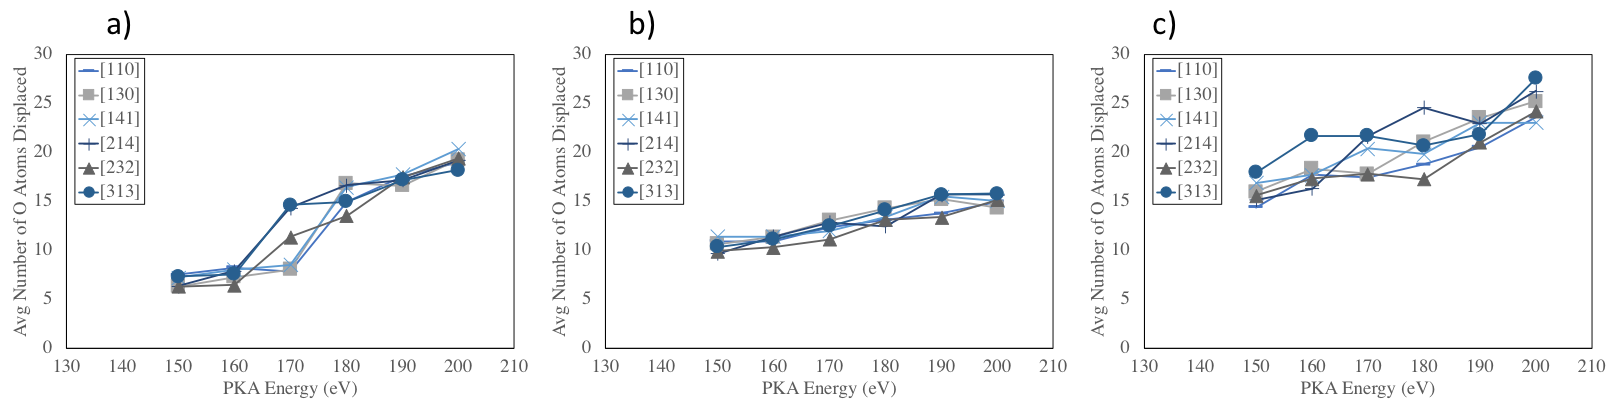
\includegraphics[width=1.0\textwidth]{dispO_OE.png}
 \caption{Average number of oxygen atoms displaced by an O PKA as a function of PKA energy in $UO_2$ in the [110], [130], [141], [214], [232] and [313] directions for the a) Basak, b) Yakub and c) Yamada potentials.  }
 \label{fig:dispoe}
\end{figure*}


\section{Discussion}

This work has shown a consistency regarding the variation among the three interatomic potentials, in that they are in concordance when considering U PKAs, but the radiation damage properties vary significantly for the Yamada potential when considering O PKAs and the O sublattice. This is likely due to the oxygen sublattice properties defined by the Yamada potential. The Yamada potential exhibits properties of a more fluid oxygen sublattice, with significant distortion of O atoms off of the sublattice, in addition to rapid O interstitial diffusion. This was visually confirmed to be the case by use of Ovito \cite{ovito}. Because the Basak potential is considered an improvement of the Yamada potential \cite{basak}, and the Basak results generally agree with the Yakub potential, the Yamada potential is viewed as producing inaccurate oxygen sublattice behavior, and the authors would discourage the use of the Yamada potential in high temperature radiation damage studies.

\section{Conclusion}
\hspace{5mm}

Molecular dynamics simulations of low energy PKAs have been performed to investigate the threshold displacement energy ($E_d$) in $UO_2$ at 1500 K. The Basak, Yakub and Yamada interatomic potentials were utilized. The $E_d$ was studied by looking at the probability of Frenkel pair production, the probability that the PKA leaves its lattice site and the number of permanently displaced atoms due to the PKA. Both uranium and oxygen PKAs were utilized to investigate a broad scope of potential radiation damage in $UO_2$. Utilizing the definition of $E_d$ as the minimum energy required to form a stable Frenkel pair, it was found that the $E_d$ for U PKAs is 25-30 eV and the $E_d$ for O PKAs is 20-30 eV, depending on the interatomic potential utilized. These results are in agreement with experimental results for O atoms, but suggest a lower $E_d$ than the experimental value of 40 eV for U atoms. For utilization of the NRT equation, a median, directionally-averaged $E_d$ for U PKAs was calculated as approximately 55 eV. This quantity was not determined for O PKAs. It was found that the PKA energy required to permanently displace an O atom from its lattice site is approximately 20 eV, regardless of the PKA type. Additionally, it requires 30 eV of kinetic energy for a U PKA to permanently displace a U atom from its lattice site. The minimum PKA energy observed for an O atom to displace a U atom is 150 eV. The results for the Basak and Yakub potentials were consistent for both U and O PKAs and showed only minimal variance across all simulated systems. The Yamada potential showed significant differences when compared to the Basak and Yakub potentials regarding O PKAs and properties of the O sublattice. This work has provided the first insight into the high temperature nature of the threshold displacement energy in $UO_2$.


\bibliographystyle{ieeetr}
\bibliography{ref}

\end{document}
